\documentclass[xcolor=tex,dvipsnames]{beamer}  % for hardcopy add 'trans'

\mode<presentation>
{
  \usetheme{Singapore}
  % or ...
  \setbeamercovered{transparent}
  % or whatever (possibly just delete it)
}


\usepackage{fontspec} 
\usepackage[mathscr]{euscript} 
%\usepackage[xcharter]{newtxmath}
%\setmainfont{XCharter}
\setmonofont{DejaVu Sans Mono}[Scale=MatchLowercase] % provides unicode characters 


\usefonttheme{professionalfonts}
%\usepackage[english]{babel}
% or whatever
%\usepackage[latin1]{inputenc}
% or whatever
%\usepackage{times}
\usepackage[T1]{fontenc}
% Or whatever. Note that the encoding and the font should match. If T1
% does not look nice, try deleting the line with the fontenc.

%%%%%%%%%%%%%%%%%%%%%% start my preamble %%%%%%%%%%%%%%%%%%%%%%
\renewcommand{\insertnavigation}[1]{}

\addtobeamertemplate{navigation symbols}{}{%
    \usebeamerfont{footline}%
    \usebeamercolor[fg]{footline}%
    \hspace{1em}%
    \insertframenumber/\inserttotalframenumber
}

\setbeamercolor{footline}{fg=blue}
\setbeamerfont{footline}{series=\bfseries}

%\setbeamertemplate{mini frames}{}

\usepackage{adjustbox}

\usepackage{graphicx}
\usepackage{amsmath, amssymb, amsthm}

\usepackage{fancyvrb}

\usepackage{hyperref}

% fonts, caligraphic
\usepackage{mathpazo}
%\usepackage{mathrsfs}
\usepackage{bbm}

% tikz
\usepackage{tikz}
\usetikzlibrary{positioning}
\usetikzlibrary{arrows}
\usetikzlibrary{calc}
\usetikzlibrary{intersections}
\usetikzlibrary{matrix}
\usetikzlibrary{decorations}
\usepackage{pgf}
\usepackage{pgfplots}
\usetikzlibrary{shapes, fit}

% from fazeleh
\usetikzlibrary{arrows.meta}

%\usetikzlibrary{arrows.meta}
\usetikzlibrary{decorations.pathreplacing}  %for brac



\usepackage{graphviz}

%\usepackage[usenames, dvipsnames]{color}


% nice inequalities
\renewcommand{\leq}{\leqslant}
\renewcommand{\geq}{\geqslant}


\setlength{\parskip}{1.5ex plus0.5ex minus0.5ex}
\setlength{\jot}{12pt} 

\usepackage[ruled, lined]{algorithm2e}


\definecolor{pale}{RGB}{235, 235, 235}
\definecolor{pale2}{RGB}{175,238,238}
\definecolor{turquois4}{RGB}{0,134,139}
\definecolor{DarkOrange1}{RGB}{255,127,0}

\newcommand{\emp}[1]{\textcolor{DarkOrange1}{\bf #1}}
\newcommand{\newtopic}[1]{\textcolor{Green}{\Large \bf #1}}
\newcommand{\navy}[1]{\textcolor{Blue}{\bf #1}}
\newcommand{\navymth}[1]{\textcolor{Blue}{#1}}
\newcommand{\red}[1]{\textcolor{red}{#1}}
\newcommand{\brown}[1]{\textcolor{Brown}{\sf #1}}
\newcommand{\green}[1]{\textcolor{ForestGreen}{\sf #1}}

% Minted
\definecolor{bg}{rgb}{0.95,0.95,0.95}
\usepackage{minted}
\usemintedstyle{friendly}
\newminted{python}{mathescape,frame=lines,framesep=4mm,bgcolor=bg}
\newminted{ipython}{mathescape,frame=lines,framesep=4mm,bgcolor=bg}
\newminted{julia}{mathescape,frame=lines,framesep=4mm,bgcolor=bg}
\newminted{c}{mathescape,frame=lines,framesep=4mm,bgcolor=bg}
\renewcommand{\theFancyVerbLine}{\sffamily
    \textcolor[rgb]{0.5,0.5,1.0}{\scriptsize {\arabic{FancyVerbLine}}}}


\newcommand{\Fact}{\textcolor{Brown}{\bf Fact. }}
\newcommand{\Facts}{\textcolor{Brown}{\bf Facts }}
\newcommand{\keya}{\textcolor{turquois4}{\bf Key Idea. }}
\newcommand{\Factnodot}{\textcolor{Brown}{\bf Fact }}
\newcommand{\Eg}{\textcolor{ForestGreen}{Example. }}
\newcommand{\Egs}{\textcolor{ForestGreen}{Examples. }}
\newcommand{\Ex}{{\bf Ex. }}



\newcommand{\CC}{\mathbbm C}
\newcommand{\EE}{\mathbbm E}
\newcommand{\FF}{\mathbbm F}
\newcommand{\RR}{\mathbbm R}
\newcommand{\KK}{\mathbbm K}
\newcommand{\MM}{\mathbbm M}
\newcommand{\NN}{\mathbbm N}
\newcommand{\PP}{\mathbbm P}
\newcommand{\TT}{\mathbbm T}
\newcommand{\QQ}{\mathbbm Q}
\newcommand{\WW}{\mathbbm W}
\newcommand{\VV}{\mathbbm V}
\newcommand{\ZZ}{\mathbbm Z}

\newcommand{\Asf}{\mathsf A}
\newcommand{\Esf}{\mathsf E}
\newcommand{\Fsf}{\mathsf F}
\newcommand{\Gsf}{\mathsf G}
\newcommand{\Msf}{\mathsf M}
\newcommand{\Lsf}{\mathsf L}
\newcommand{\Nsf}{\mathsf N}
\newcommand{\Psf}{\mathsf P}
\newcommand{\Qsf}{\mathsf Q}
\newcommand{\Ssf}{\mathsf S}
\newcommand{\Tsf}{\mathsf T}
\newcommand{\Xsf}{\mathsf X}
\newcommand{\Ysf}{\mathsf Y}
\newcommand{\Vsf}{\mathsf V}
\newcommand{\Wsf}{\mathsf W}
\newcommand{\Zsf}{\mathsf Z}

\newcommand{\aA}{\mathscr A}
\newcommand{\bB}{\mathscr B}
\newcommand{\cC}{\mathscr C}
\newcommand{\dD}{\mathscr D}
\newcommand{\eE}{\mathscr E}
\newcommand{\gG}{\mathscr G}
\newcommand{\hH}{\mathscr H}
\newcommand{\iI}{\mathscr I}
\newcommand{\fF}{\mathscr F}
\newcommand{\lL}{\mathscr L}
\newcommand{\pP}{\mathscr P}
\newcommand{\rR}{\mathscr R}
\newcommand{\sS}{\mathscr S}
\newcommand{\vV}{\mathscr V}
\newcommand{\wW}{\mathscr W}
\newcommand{\mM}{\mathscr M}
\newcommand{\oO}{\mathscr O}
\newcommand{\zZ}{\mathscr Z}

\newcommand{\bP}{\mathbf P} 
\newcommand{\bR}{\mathbf R}
\newcommand{\bQ}{\mathbf Q}


%%%%%% special symbols %%%%%%%%%%

\newcommand{\volone}{Volume~I}
\newcommand{\voltwo}{Volume~II}

% transpose, not currently using
\newcommand\T{{\mathpalette\raiseT\intercal}}
\newcommand\raiseT[2]{\raisebox{0.25ex}{$#1#2$}}

% nice inequalities
\renewcommand{\leq}{\leqslant}
\renewcommand{\geq}{\geqslant}

% nice greek letters
\renewcommand{\phi}{\varphi}
\renewcommand{\epsilon}{\varepsilon}

% inner product
\providecommand{\inner}[1]{\left\langle{#1}\right\rangle}

% set of matrices
\newcommand{\matset}[2]{ \MM^{ #1 \times #2 } }

% stochastic dominance
\newcommand{\lefsd}{\preceq_{\textrm{F}}}
\newcommand{\lessd}{\preceq_{\textrm{S}}}

% argmax and min
\newcommand{\argmax}{\operatornamewithlimits{argmax}}
\newcommand{\argmin}{\operatornamewithlimits{argmin}}

% sets and logic
\newcommand{\st}{\ensuremath{\ \mathrm{s.t.}\ }}
\newcommand{\setntn}[2]{ \{ #1 : #2 \} }
\newcommand{\natset}[1]{[ #1 ]}

% some useful symbols
\newcommand{\given}{\, | \,}
\newcommand{\cf}[1]{ \lstinline|#1| }
\newcommand{\fore}{\therefore \quad}
\newcommand{\1}{\mathbbm 1}
\newcommand{\me}{\mathrm{e}}               % Euler's e
\newcommand*\diff{\mathop{}\!\mathrm{d}}   % d for integrals

% shortcuts
\newcommand{\la}{\langle}
\newcommand{\ra}{\rangle}

% relations
\newcommand{\eqdist}{\stackrel{d} {=} }
\newcommand{\iidsim}{\stackrel{\textrm{ {\sc iid }}} {\sim} }

% convergence
\newcommand{\tod}{\stackrel { d } {\to} }
\newcommand{\tow}{\stackrel { w } {\to} }
\newcommand{\toprob}{\stackrel { p } {\to} }
\newcommand{\toms}{\stackrel { ms } {\to} }


%%%%%%%%%%% operators %%%%%%%%%%%%

\DeclareMathOperator{\Exp}{Exp}  % exponential draw
\DeclareMathOperator{\Lip}{Lip}
\DeclareMathOperator{\cl}{cl}
\DeclareMathOperator{\graph}{graph}
\DeclareMathOperator{\interior}{int}
\DeclareMathOperator{\Prob}{Prob}
\DeclareMathOperator{\determinant}{det}
\DeclareMathOperator{\trace}{trace}
\DeclareMathOperator{\sgn}{sgn}
\DeclareMathOperator{\Span}{span}
\DeclareMathOperator{\diag}{diag}
\DeclareMathOperator{\proj}{proj}
\DeclareMathOperator{\rank}{rank}
\DeclareMathOperator{\kernel}{null}
\DeclareMathOperator{\cov}{Cov}
\DeclareMathOperator{\corr}{Corr}
\DeclareMathOperator{\var}{Var}
\DeclareMathOperator{\mse}{mse}
\DeclareMathOperator{\se}{se}
\DeclareMathOperator{\range}{range}
\DeclareMathOperator{\dimension}{dim}
\DeclareMathOperator{\epi}{epi}
\DeclareMathOperator{\vecop}{vec}

\DeclareMathOperator{\real}{Re}
\DeclareMathOperator{\imag}{Im}

\DeclareMathOperator{\csum}{cs} % column sum
\DeclareMathOperator{\rsum}{rs} % row sum



\hypersetup{
    linkcolor=Blue,
    colorlinks=true,
    filecolor=magenta,      % color of file links
    urlcolor=cyan           % color of external links
}


%\pgfdeclareimage[height=1.2cm]{university-logo}{../tuxswatter2}
%\logo{\pgfuseimage{university-logo}}

%\addtobeamertemplate{headline}{}
%{%
%\begin{flushright}
%\begin{tikzpicture}[remember picture,overlay]
%\node [left ]{\includegraphics[width=0.5cm]{../tuxswatter2.png}};
%\end{tikzpicture}
%\end{flushright}
%\vskip -0.1cm
%} 

 \date[\today]{}

\title{CBC QuantEcon Workshop}







\subtitle{Prelude to Dynamic Programming}

\author{John Stachurski}

\date{September 2022}


\begin{document}

\begin{frame}
  \titlepage
\end{frame}


\section{Introduction}


\begin{frame}
    \frametitle{Introduction}

    Summary of this lecture:

    \begin{itemize}
        \item Linear equations
            \vspace{0.3em}
        \item Fixed point theory
            \vspace{0.3em}
        \item Algorithms
            \vspace{0.3em}
        \item Job search
    \end{itemize}

            \vspace{0.3em}
            \vspace{0.3em}

    Resources:
    %
    \begin{itemize}
        \item Slides and DP textbook at \url{https://github.com/jstac/paris_workshop_2022}
    \end{itemize}

    %\emp{Lecture slides at} \url{https://github.com/jstac/tokyo_2022_coursework}

\end{frame}



%\begin{frame}
    
    %Convention: Real operations extend to vectors \underline{element-by-element}

    %\vspace{1em}
    %\Eg
    %%
    %\begin{equation*}
        %a = 
        %\begin{pmatrix}
            %a_1 \\
            %\vdots \\
            %a_n
        %\end{pmatrix}
        %\quad \implies \quad
        %|a| = 
        %\begin{pmatrix}
            %|a_1| \\
            %\vdots \\
            %|a_n|
        %\end{pmatrix}
    %\end{equation*}
    %%

    %\vspace{1em}

    %%
    %\begin{equation*}
        %a \vee b = 
        %\begin{pmatrix}
            %a_1 \vee b_1 \\
            %\vdots \\
            %a_n \vee b_n 
        %\end{pmatrix}
    %\end{equation*}
    %%

    %etc.

%\end{frame}



\section{Fixed Point Theory}

\begin{frame}
     \frametitle{Linear Equations}   

    For scalar equation $x = ax + b$, 
    %
    \begin{align*}
        |a| < 1 \quad \implies \quad
        x^* & = \frac{b}{1-a} \\
            & = \sum_{i \geq 0} a^i b
    \end{align*}
    %

    How can we extend this beyond one dimension?

    \vspace{1em}
    \begin{itemize}
        \item When does $x = Ax + b$ have a unique solution?
        \vspace{1em}
        \item How can we compute it?
    \end{itemize}

\end{frame}


\begin{frame}

    Recall that $\lambda \in \CC$ is an \navy{eigenvalue} of $n \times n$ matrix $A$ if
    %
    \begin{equation*}
        A e = \lambda e
        \quad \text{for some nonzero $e \in \CC^n$}
    \end{equation*}
    %

    \vspace{1em}
    We define the \navy{spectral radius} of $A$ as
    %
    \begin{equation*}
        r(A) := \max\setntn{|\lambda|}{\lambda \text{ is an eigenvalue of } A}    
    \end{equation*}
    %

    \vspace{1em}
    \vspace{1em}
    \emp{Key idea}: 
    %
    \begin{itemize}
        \item $r(A)<1$ is a generalization of $|a|<1$
    \end{itemize}



    
\end{frame}

\begin{frame}
    \frametitle{Neumann Series Lemma}

    Suppose 
    %
    \begin{itemize}
        \item $b$ is $n \times 1$ and $A$ is $n \times n$ 
        \item $I$ is the $n \times n$ identity matrix
    \end{itemize}

    \vspace{0.5em}

    \vspace{0.5em}
    {\bf Theorem.} 
    If $r(A) < 1$, then
    %
    \begin{enumerate}
        \item $I - A$ is nonsingular 
        \vspace{0.5em}
        \item $\sum_{k \geq 0} A^k$ converges 
        \vspace{0.5em}
        \item $(I - A)^{-1} = \sum_{k \geq 0} A^k$ and
        \vspace{0.5em}
        \item $x = A x + b$ has the unique solution 
            %
            \begin{equation*}
                x^* := (I - A)^{-1} b 
            \end{equation*}
            %
    \end{enumerate}

    
\end{frame}

\begin{frame}
    
    Intuitive idea: with $S := \sum_{k \geq 0} A^k$, we have
    %
    \begin{align*}
        I + AS 
        & = I + A (I + A + \cdots)
        \\
        & = I + A + A^2 + \cdots 
        \\
        & = S
    \end{align*}
    %

    Rearranging $I + AS = S$ gives $S = (I - A)^{-1}$
            \vspace{0.5em}
            \vspace{0.5em}

    \begin{equation*}
        \fore
        x = Ax + b
        \; \iff \; 
        (I - A)x = b
        \; \iff \; 
        x^* = (I-A)^{-1} b
    \end{equation*}


\end{frame}


\begin{frame}
    \frametitle{Fixed points}    

    To solve \underline{nonlinear} equations we use fixed point theory

            \vspace{0.4em}
            \vspace{0.4em}
    Recall: if $S$ is any set then
    %
    \begin{itemize}
        \item $T$ is a \navy{self-map} on $S$ if $T$ maps $S$ into itself
            \vspace{0.4em}
        \item  $x^* \in S$ is called a
            \navy{fixed point} of $T$ in $S$ if $T x^* = x^*$  
    \end{itemize}

            \vspace{0.4em}
            \vspace{0.4em}
    \Egs 
    %
    \begin{itemize}
        \item Every $x$ in $S$ is fixed for the \navy{identity map}
            $I \colon x \mapsto x$
            \vspace{0.4em}
        \item If $S = \NN$ and $Tx = x+1$, then $T$ has no fixed point
    \end{itemize}


\end{frame}


\begin{frame}
    
    \Eg
    %
    \begin{itemize}
        \item If $S \subset \RR$, then  $Tx =x$ $\iff$ $T$ meets the 45 degree line
    \end{itemize}


\end{frame}



\begin{frame}
    
    \begin{figure}
        \centering
        \scalebox{0.45}{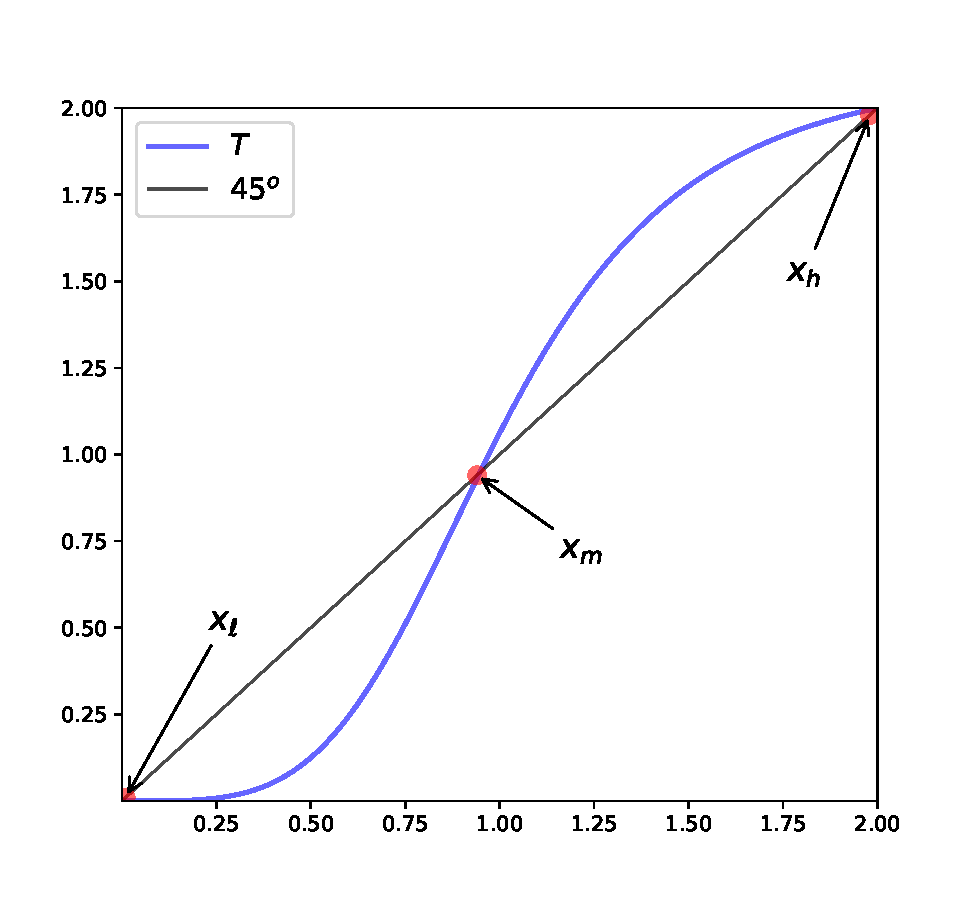
\includegraphics{local_figs/three_fixed_points.pdf}}
        \caption{\label{f:three_fixed_points} 
            Graph and fixed points of $T \colon x \mapsto 2.125/(1 + x^{-4})$ }
    \end{figure}

\end{frame}


\begin{frame}

    \emp{Key idea}: Fixed point theory is for solving equations

    \vspace{1em}
    \vspace{1em}

    \Eg If $S = \RR^n$ and $T x = Ax + b$, then 
    %
    \begin{center}
        $x^*$ solves equation  $x = Ax + b$
        $\iff$ 
        $x^*$ is a fixed point of $T$ 
    \end{center}


    \vspace{1em}

    \Eg  If $G \colon \RR^n \to \RR^n$, then
    %
    \begin{center}
        solve $Gx = 0$ $\iff$ find fixed points of $Tx = Gx + x$
    \end{center}

    
\end{frame}


\begin{frame}
    
    Point on notation:
    %
    \begin{itemize}
        \item $T^2 = T \circ T$
            \vspace{0.4em}
        \item $T^3 = T \circ T \circ T$
            \vspace{0.4em}
        \item etc.
    \end{itemize}
            \vspace{0.4em}
            \vspace{0.4em}
            \vspace{0.4em}


    \Eg $Tx = Ax + b$ implies $T^2x = A(Ax + b) + b$

\end{frame}



\begin{frame}
    
    Self-map $T$ is called \navy{globally stable} on $S$
    if 
    %
    \begin{enumerate}
        \item $T$ has a unique fixed point $x^*$ in $S$ and
            \vspace{0.4em}
        \item $T^k x \to x^*$ as $k \to \infty$ for all $x \in S$  
    \end{enumerate}

    \vspace{1em}
    \vspace{1em}

    \Eg Let $S = \RR^n$ and $Tx = Ax + b$

            \vspace{0.4em}
    \Ex Prove: $r(A) < 1$ implies $T$ is globally stable on $S$

\end{frame}



\begin{frame}
    
    \Eg Consider Solow--Swan growth dynamics 
    %
    \begin{equation*}
        \label{eq:solow}
        k_{t+1} = g(k_t) := s A k_t^\alpha + (1 - \delta) k_t,
        \qquad t = 0, 1, \ldots,
    \end{equation*}
    %
    where 
    %
    \begin{itemize}
        \item $k_t$ is capital stock per worker,
        \item $A, \alpha >0$ are production parameters, $\alpha < 1$
        \item $s > 0$ is a savings rate, and
        \item $\delta \in (0,1)$ is a rate of depreciation  
    \end{itemize}

    Iterating with $g$ from $k_0$ generates a time path for capital stock

    The map $g$ is globally stable on $(0, \infty)$

\end{frame}

\begin{frame}
    
    \begin{figure}
       \centering
       \scalebox{0.6}{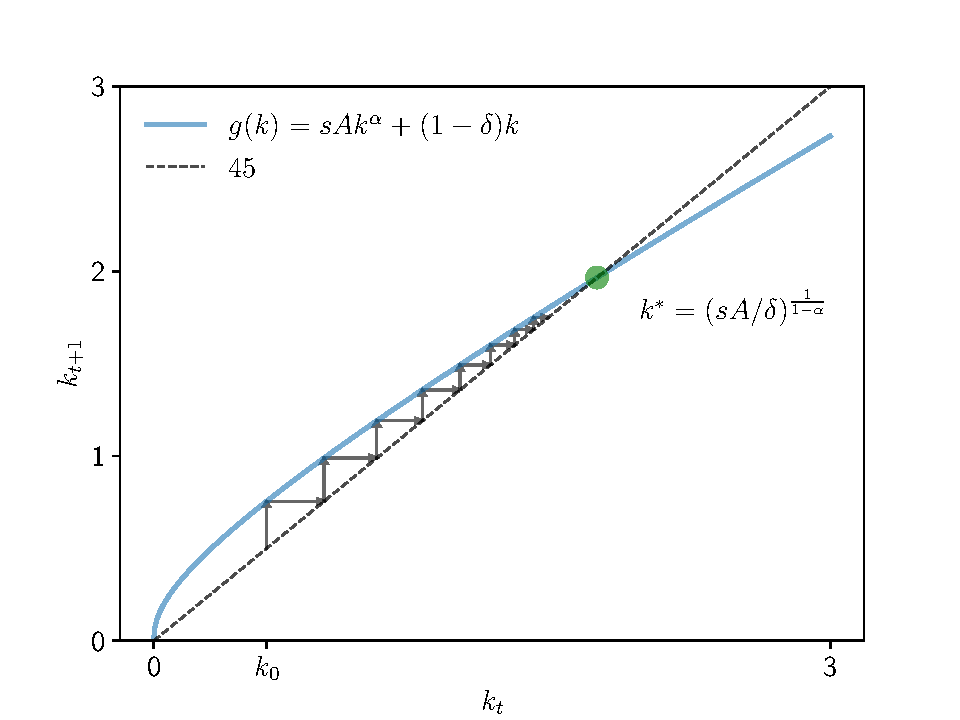
\includegraphics{local_figs/solow_fp_1.pdf}}
    \end{figure}

\end{frame}

\begin{frame}
    
    \begin{figure}
       \centering
       \scalebox{0.6}{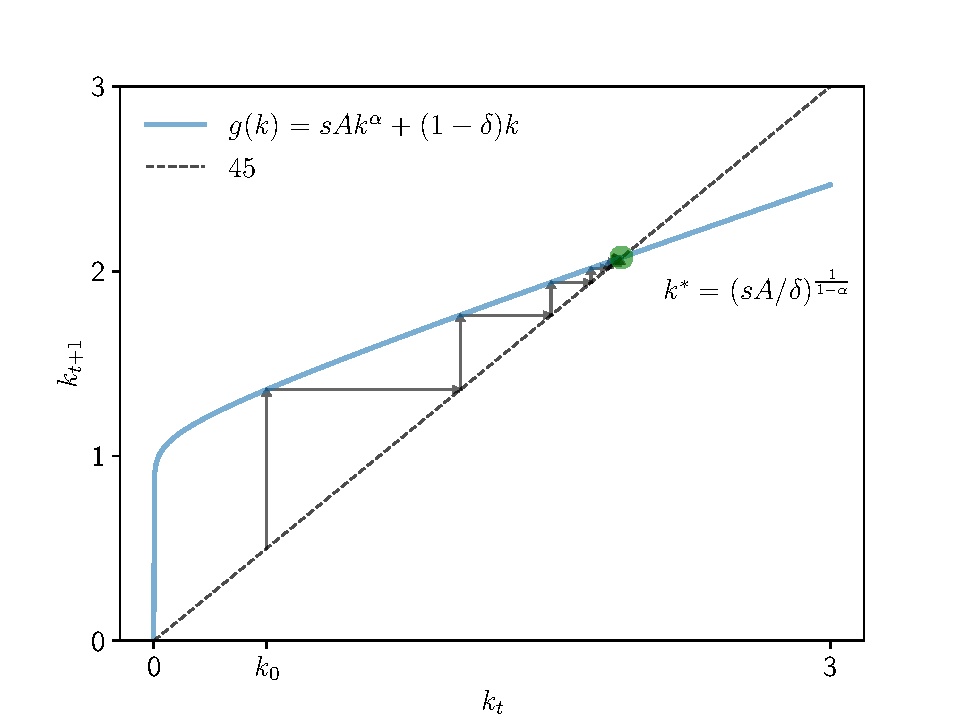
\includegraphics{local_figs/solow_fp_2.pdf}}
    \end{figure}

\end{frame}


\begin{frame}
    
    Note from last slide

    \begin{itemize}
        \item If $g$ is flat near $k^*$, then $g(k) \approx k^*$ for $k$ near $k^*$
    \vspace{0.3em}
        \item A flat function near the fixed point $\implies$ fast convergence
    \end{itemize}

    \vspace{0.3em}
    \vspace{0.3em}
    Conversely

    \begin{itemize}
        \item If $g$ is close to the 45 degree line near $k^*$, then $g(k)
            \approx k$ 
    \vspace{0.3em}
        \item Close to 45 degree line means high persistence, slow convergence
    \end{itemize}
    %


\end{frame}




\begin{frame}

    Under what conditions are self-maps globally stable?

\end{frame}

\begin{frame}
    \frametitle{Contractions}
    
    Let 
    %
    \begin{itemize}
        \item $U$ be a nonempty subset of $\RR^n$
    \vspace{0.3em}
    \vspace{0.3em}
        \item $\| \cdot \|$ be a norm on $\RR^n$
    \vspace{0.3em}
    \vspace{0.3em}
        \item $T$ be a self-map on $U$

    \end{itemize}

    \vspace{0.3em}
    \vspace{0.3em}
    \vspace{0.3em}
    $T$ is called a \navy{contraction} on $U$ with respect
    to $\| \cdot \|$ if 
    %
    \begin{equation*}
        \text{$\exists \, \lambda < 1$ such that }
        \| Tu - Tv \| \leq \lambda \| u - v \| \quad \text{for all} \quad u, v \in U
    \end{equation*}
    %

    %\Eg $Tx = ax + b$ is a contraction on $\RR$ with respect to $| \cdot |$ 
    %if and only if $|a|<1$

    %Indeed, 
    %%
    %\begin{equation*}
        %|Tx - Ty| = |ax + b - ay - b| = |a| |x -y|
    %\end{equation*}
    


\end{frame}




\begin{frame}
    \frametitle{Banach's contraction mapping theorem}
    
    {\bf Theorem} If 
    %
    \begin{enumerate}
        \item $U$ is closed in $\RR^n$ and
        \item $T$ is a contraction of modulus $\lambda$ on $U$
        with respect to some norm $\| \cdot \|$ on $\RR^n$,
    \end{enumerate}
    %
    then $T$ has a unique fixed point $u^*$ in $U$ and 
    %
    \begin{equation*}
        \| T^n u - u^* \| \leq \lambda^n \| u - u^* \|
        \quad \text{for all } n \in \NN \text{ and } u \in U
    \end{equation*}
    %
    In particular, $T$ is globally stable on $U$


\end{frame}


\begin{frame}
    \frametitle{Successive approximation}

    \vspace{0.3em}
    \begin{algorithm}[H]
      \DontPrintSemicolon
      fix a guess $x_0$ and some error tolerance $\tau$ \;
      $\epsilon \leftarrow \tau + 1$ \;
      $x \leftarrow x_0$ \;
      \While{$\epsilon > \tau$}
      {
          $y \leftarrow T x$ \;
          $\epsilon \leftarrow \| y - x \|$ \;
          $x \leftarrow y$ \;
      }
      \Return{$x$}
    \end{algorithm}

    \vspace{0.3em}
    \vspace{0.3em}
    \underline{If} $T$ is a contraction, say, then the output will be close to
    to $x^*$

    
\end{frame}


\begin{frame}
    
    \begin{listing}[H]
    \inputminted[
        firstline=1,
        frame=lines,
        framesep=1em,
        %bgcolor=codebg,
        fontsize=\scriptsize
        ]{python}{../../solvers.py} 
    \end{listing}

\end{frame}

\begin{frame}
    

    \begin{figure}
        \centering
        \scalebox{0.52}{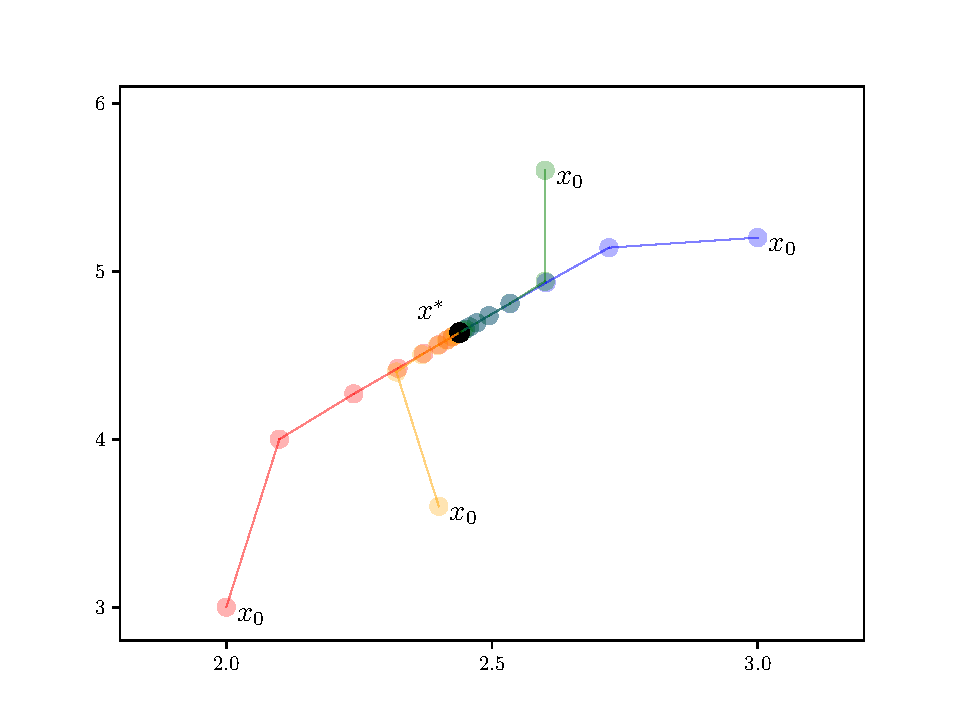
\includegraphics{local_figs/linear_iter_fig_1.pdf}}
        \caption{\label{f:linear_iter_fig_1} 
            Successive approximation from different initial conditions}
    \end{figure}

\end{frame}


\begin{frame}
    \frametitle{Newton's Method}

    \vspace{0.3em}
    Let $g$ be a smooth self-map on $S := (a, b)$ 

    \vspace{0.3em}
    \vspace{0.3em}
    We start with guess $x_0$ of the fixed point and define
    %
    $$\hat g(x) \approx g(x_0) + g'(x_0)(x - x_0)$$

    \vspace{0.3em}
    Set $\hat g(x_1) = x_1$ and solve for $x_1$ to get
    %
    \begin{equation*}
        x_1 = \frac{g(x_0) - g'(x_0) x_0}{1 - g'(x_0)}
    \end{equation*}

\end{frame}


\begin{frame}

    \begin{figure}
       \centering
       \scalebox{0.5}{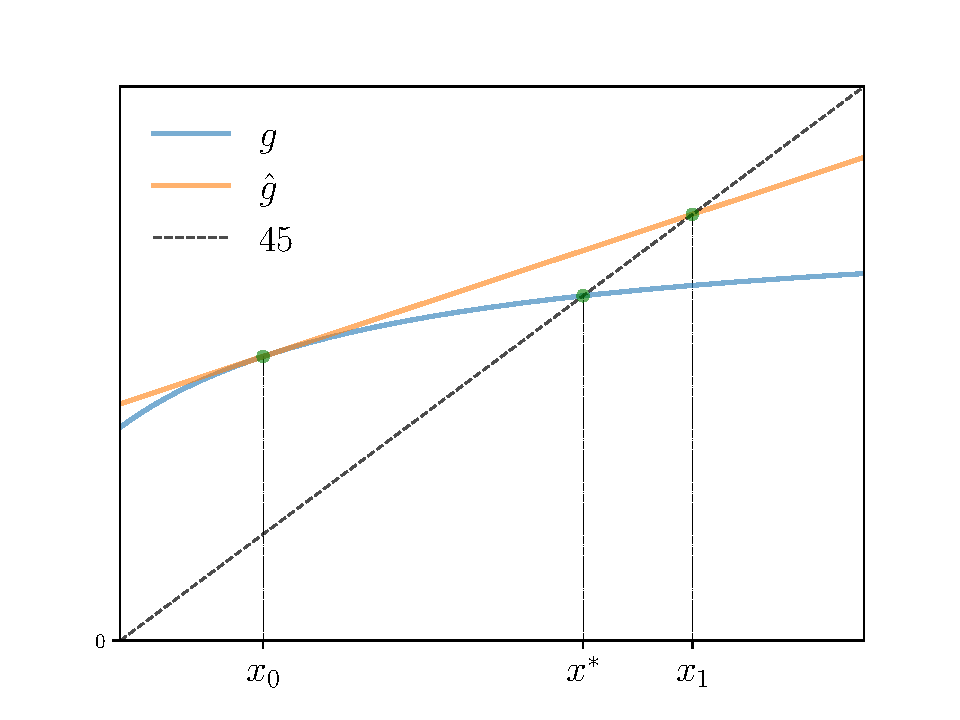
\includegraphics{local_figs/newton_1.pdf}}
       \caption{\label{f:newton_1} The first step of Newton's method applied to $g$}
    \end{figure}

\end{frame}

\begin{frame}

    Now repeat logic to get $x_2, x_3, \ldots $
    \vspace{0.3em}
    \vspace{0.3em}

    In other words, we iterate on $x_{k+1} = q(x_k)$ where
    
    \begin{equation*}
        q(x) := \frac{g(x) - g'(x) x}{1 - g'(x)}
    \end{equation*}
    %

    \vspace{0.3em}
    \vspace{0.3em}
    \vspace{0.3em}
    \vspace{0.3em}
    Note:
    \begin{itemize}
        \item we are applying successive approximation to $q$
        \vspace{0.3em}
        \vspace{0.3em}
        \item Hence we can use the same code
    \end{itemize}



\end{frame}


\begin{frame}
    
    \begin{figure}
       \centering
       \scalebox{0.5}{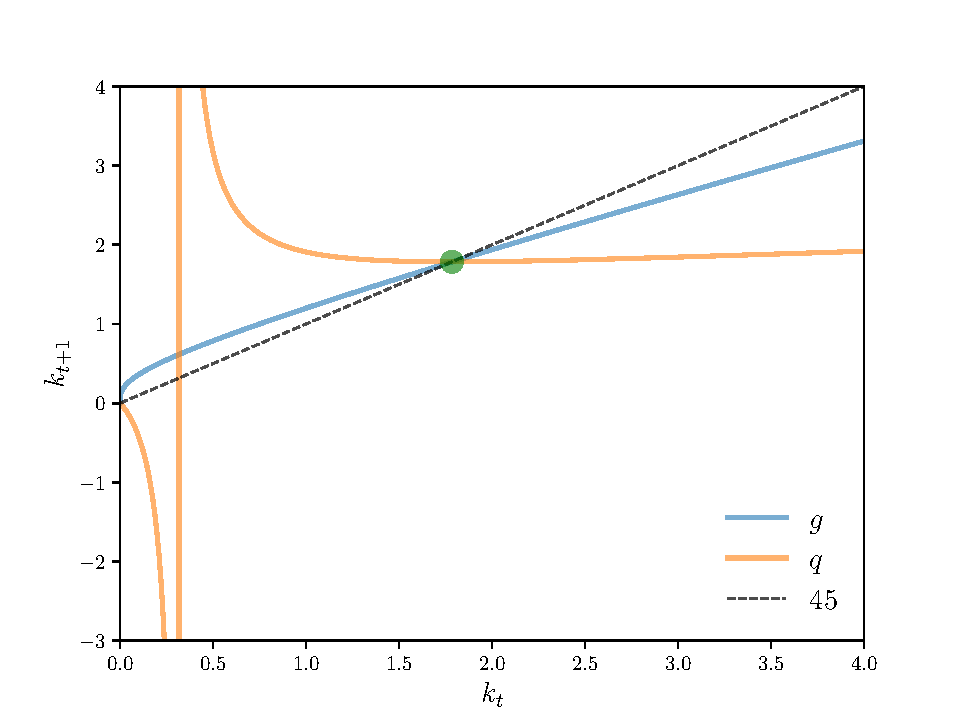
\includegraphics{local_figs/newton_solow_45.pdf}}
       \caption{\label{f:newton_solow_45} Successive approximation vs Newton's method}
    \end{figure}

\end{frame}

\begin{frame}
    
    Comments:
    %
    \begin{itemize}
        \item The map $q$ is flat close to the fixed point $k^*$
            \vspace{0.5em}
        \item Hence Newton's method converges quickly \underline{near} $k^*$
            \vspace{0.5em}
        \item But Newton's method is not globally convergent
            \vspace{0.5em}
        \item Successive approximation is slower but more robust
    \end{itemize}


    \emp{Key ideas}
    %
    \begin{itemize}
        \item There is almost always a trade-off between robustness and speed
            \vspace{0.5em}
        \item Speed requires assumptions, and assumptions can fail
    \end{itemize}


\end{frame}


\begin{frame}
    
    \emp{Newton's method} extends naturally to \emp{multiple dimensions}

            \vspace{0.5em}
    When $h$ is a map from $S \subset \RR^n$ to itself, we use

    %
    \begin{equation*}
        x_{k+1} = x_k - [J(x_k)]^{-1} h(x_k)
    \end{equation*}
    %

    Here $J_h(x_k) := $ the Jacobian of $h$ evaluated at $x_k$

    \vspace{1em}

    Comments
    %
    \begin{itemize}
        \item Typically faster but less robust
            \vspace{0.5em}
        \item Matrix operations can be parallelized
            \vspace{0.5em}
        \item Automatic differentiation can be helpful
    \end{itemize}



\end{frame}


\begin{frame}
    
    See the notebook \texttt{solow\_fixed\_points.ipynb}

\end{frame}



\begin{frame}
    \frametitle{Job Search}

    A model of job search created by \emp{John J. McCall}
    \vspace{0.5em}

    We model the \underline{decision problem of an unemployed worker}

    \vspace{0.5em}
    Job search depends on
    %
    \begin{itemize}
        \item current and likely future wage offers
    \vspace{0.5em}
        \item impatience, and
    \vspace{0.5em}
        \item the availability of unemployment compensation
    \end{itemize}

    \vspace{0.5em}
    We use a very simple version of the McCall model 

\end{frame}


\begin{frame}
    \frametitle{Set Up}
    
    An agent begins working life unemployed at $t=0$ 

            \vspace{0.5em}
    Receives a new job offer paying wage $W_t$ at each date $t$  
            \vspace{0.5em}
            \vspace{0.5em}

    Two choices:
    %
    \begin{enumerate}
        \item \emp{accept} the offer and work \underline{permanently} at $W_t$ or
            \vspace{0.5em}
        \item \emp{reject} the offer, receive unemployment compensation $c$, and reconsider next period
    \end{enumerate}

            \vspace{0.5em}
            \vspace{0.5em}
    \begin{itemize}
        \item $\{ W_t \} \iidsim \phi$ for $\phi \in \dD(\Wsf)$ where $\Wsf
            \subset \RR_+$ with $|\Wsf| < \infty$
    \end{itemize}


\end{frame}



\begin{frame}

    The agent lives forever (infinite horizon) but is \emp{impatient}

            \vspace{0.5em}
    Impatience is parameterized by a \navy{time discount factor} $\beta \in (0, 1)$

            \vspace{0.5em}
    \begin{itemize}
        \item Present value of a next-period payoff of $y$ dollars is $\beta y$
    \end{itemize}

            \vspace{0.5em}
            \vspace{0.5em}
    Trade off:
    %
    \begin{itemize}
        \item $\beta < 1$ indicating some impatience
            \vspace{0.5em}
        \item hence the agent will be
            tempted to accept reasonable offers, rather than always waiting
            for a better one
            \vspace{0.5em}
        \item The key question is how long to wait
    \end{itemize}
   
\end{frame}



\begin{frame}
    
    The worker aims to maximize expected present value (EPV) of earnings

        \vspace{0.4em}
    If we \emp{accept} $w \in \Wsf$,
    %
    \begin{equation*}
        \text{EPV }
        = \text{stopping value }
        = w + \beta w + \beta^2 w + \cdots 
        = \frac{w}{1 - \beta}
    \end{equation*}
    %    

        \vspace{0.4em}
    If we \emp{reject},
    %
    \begin{align*}
        \text{EPV }
        & = \text{continuation value }
        \\
        & = \text{$c$ + $\beta \times$ EPV of 
        \underline{optimal} choices in subsequent periods}
    \end{align*}

        \vspace{0.4em}
    But what are optimal choices?!
        \vspace{0.4em}

    Calculating optimal choice requires knowing optimal choice!

\end{frame}

\begin{frame}
    \frametitle{The Value Function}

    Let  $v^*(w) :=$ max lifetime EPV given wage offer $w$
    \vspace{0.4em}

    We call $v^*$ the \navy{value function}\index{Value function}
    \vspace{0.4em}

    \emp{If} we know $v^*$ then we can compute the \navy{continuation value} 
    %
    \begin{equation*}
        h^* 
        := c + \beta \, \sum_{w' \in \Wsf} \, v^*(w') \phi(w') 
    \end{equation*}

    The optimal choice is then
    %
    \begin{equation*}
         \1
        \left\{
            \text{stopping value} \geq \text{continuation value}
        \right\}
         = \1
        \left\{
            \frac{w}{1 - \beta}, \; h^*
        \right\}
    \end{equation*}


    (Here 1 means ``accept'' and 0 means ``reject'')

\end{frame}


\begin{frame}

    But how can we calculate $v^*$?

    \vspace{0.4em}
    \emp{Key idea}: Use the Bellman equation 

    \vspace{0.4em}
    {\bf Theorem.} The value function $v^*$ satisfies the \navy{Bellman
    equation}
    %
    \begin{equation*}
        v^*(w) = 
        \max \left\{
            \frac{w}{1-\beta}
            ,\,
            c + \beta \, \sum_{w' \in \Wsf} \, v^*(w') \phi(w')
            \right\}
            \qquad (w \in \Wsf)
    \end{equation*}
    %

    \vspace{0.4em}
    \vspace{0.4em}
    \vspace{0.4em}
    Intuition: Max value today is max over the alternatives
    %
    \begin{enumerate}
        \item accept and get $w/(1-\beta)$
        \vspace{0.4em}
        \item reject and get max continuation value
    \end{enumerate}


\end{frame}


\begin{frame}

    So how can we use the Bellman equation
    %
    \begin{equation*}
        v^*(w) = 
        \max \left\{
            \frac{w}{1-\beta}
            ,\,
            c + \beta \, \sum_{w' \in \Wsf} \, v^*(w') \phi(w')
            \right\}
            \qquad (w \in \Wsf)
    \end{equation*}
    %
    to solve for $v^*$?


\end{frame}






%\begin{frame}

    %Let's now return to the job search problem 

    %Recall that that the value function $v^*$ solves the Bellman equation

    %\vspace{1em}

    %That is,
    %%
    %\begin{equation*}
        %v^*(w) = 
        %\max \left\{
            %\frac{w}{1-\beta}
            %,\,
            %c + \beta \, \sum_{w' \in \Wsf} \, v^*(w') \phi(w')
            %\right\}
            %\qquad (w \in \Wsf)
    %\end{equation*}
    %%

    %\vspace{1em}

    %The infinite-horizon \navy{continuation value} is defined as
    %%
    %\begin{equation*}
        %h^* := c + \beta \sum_{w'} v^*(w') \phi(w') 
    %\end{equation*}
    %%

    %\emp{Key question}: how to solve for $v^*$?  

%\end{frame}


\begin{frame}

    We introduce the \navy{Bellman operator}, defined at
    $v \in \RR^\Wsf$ by
    %
    \begin{equation*}
        (Tv)(w) 
        = 
        \max 
        \left\{
            \frac{w}{1-\beta}
            ,\,
            c + \beta \sum_{w' \in \Wsf} v(w') \phi(w')
        \right\}
        \qquad (w \in \Wsf)
    \end{equation*}
    %

    By construction, $Tv=v$ $\iff$ $v$ solves the Bellman equation 

        \vspace{0.5em}
    Let $\vV := \RR^\Wsf_+$ 

        \vspace{0.5em}
    {\bf Proposition.} $T$ is a contraction on $\vV$
        with respect to $\| \cdot \|_\infty$

        \vspace{0.5em}
    In the proof, we use the elementary bound
    %
    \begin{equation*}
        |\alpha \vee x - \alpha \vee y| \leq |x - y|
        \qquad (\alpha, x, y \in \RR)
    \end{equation*}
    %

\end{frame}


\begin{frame}
    
    Fixing $f, g$ in $\vV$ fix any $w \in \Wsf$, we have 
    %
    \begin{align*}
        |(Tf)(w) - (Tg)(w)|
        & \leq \left|
        \beta \sum_{w'} f(w') \phi(w')
                -
                \beta \sum_{w'} g(w') \phi(w')  
            \right|
        \\
        & = \beta 
            \left|
            \sum_{w'} [f(w') - g(w')] \phi(w') 
            \right|
    \end{align*}
    %

    Applying the triangle inequality,
    %
    \begin{equation*}
        |(Tf)(w) - (Tg)(w)|
        \leq \beta \sum_{w'} |f(w') - g(w')| \phi(w') 
        \leq \beta \| f - g \|_\infty 
    \end{equation*}
    %

    %
    \begin{equation*}
        \fore
        \|Tf - Tg \|_\infty \leq \beta \| f - g \|_\infty 
    \end{equation*}
    %

\end{frame}



\begin{frame}
    \frametitle{Choices as policies}
    
    %
    \begin{itemize}
        \item \navy{states} $=$ set of wage offers 
        \item possible \navy{actions} are accept (1) or reject (0)
    \end{itemize}

    A \navy{policy} is a map from states to actions

    Let $\Sigma$ be all $\sigma \colon \Wsf \to \{0, 1\}$

    For each $v \in \vV$, let us define a \navy{$v$-greedy
    policy} to be a $\sigma \in \Sigma$ satisfying
    %
    \begin{equation*}
        \sigma(w) 
        = \1
        \left\{
            \frac{w}{1-\beta}
            \geq
            c + \beta \, \sum_{w' \in \Wsf} v(w') \phi(w')
        \right\}
        \quad \text{for all } w \in \Wsf
    \end{equation*}
    %

    Accepts iff $w/(1-\beta) \geq$ continuation value computed
    using $v$ 

\end{frame}


\begin{frame}
    

    The \emp{optimal policy} is
    %
    \begin{equation*}
        \sigma^*(w) 
        = \1
        \left\{
            \frac{w}{1-\beta}
            \geq
            c + \beta \, \sum_{w' \in \Wsf} v^*(w') \phi(w')
        \right\}
        \quad \text{for all } w \in \Wsf
    \end{equation*}

    In other words
    %
    \begin{center}
        $\sigma \in \Sigma$ is optimal
        $\iff$
        $\sigma$ is $v^*$-greedy policy
    \end{center}

            \vspace{0.5em}
    This is \navy{Bellman's principle of optimality}


\end{frame}


\begin{frame}
    \frametitle{Reservation wage}
    

            \vspace{0.5em}
    We can also express a $v^*$-greedy policy via
    %
    \begin{equation*}
        \sigma^*(w) 
        = \1
        \left\{
            w \geq w^*
        \right\}
    \end{equation*}
    %

    where
    %
    \begin{equation*}
        w^* := (1 - \beta) h^* 
        \quad \text{with} \quad
        h^* 
        := c + \beta \, \sum_{w' \in \Wsf} \, v^*(w') \phi(w') 
    \end{equation*}

            \vspace{0.5em}
            \vspace{0.5em}
    The term $w^*$ is called the \navy{reservation
    wage}

    \begin{itemize}
        \item Same ideas, different language
    \end{itemize}

\end{frame}

\begin{frame}
    \frametitle{Computation}

    Since $T$ is globally stable on $\vV$, we can compute an approximate
    optimal policy as follows

            \vspace{0.5em}
    %
    \begin{enumerate}
        \item apply successive approximation on $T$ to compute $v \approx v^*$
            \vspace{0.5em}
        \item calculate a $v$-greedy policy
    \end{enumerate}

            \vspace{0.5em}
            \vspace{0.5em}
            \vspace{0.5em}
    This approach is called \navy{value function iteration}

\end{frame}



\begin{frame}

    {\small 
        \begin{algorithm}[H]
        \DontPrintSemicolon
        input $v_0 \in \vV$, an initial guess of $v^*$ \;
        input $\tau$, a tolerance level for error \;
        $\epsilon \leftarrow \tau + 1$ \;
        $k \leftarrow 0$ \;
        \While{$\epsilon > \tau $}
        {
            \For{$w \in \Wsf$}
            {
                $v_{k+1}(w) \leftarrow (Tv_k) (w)$ \;
            }
            $\epsilon \leftarrow \| v_k - v_{k+1} \|_\infty$ \;
            $k \leftarrow k + 1$ \;
        }
        Compute a $v_k$-greedy policy $\sigma$ \;
        \Return{$\sigma$}
    \end{algorithm}
    }


\end{frame}


\begin{frame}
    
    \begin{figure}
        \centering
        \scalebox{0.42}{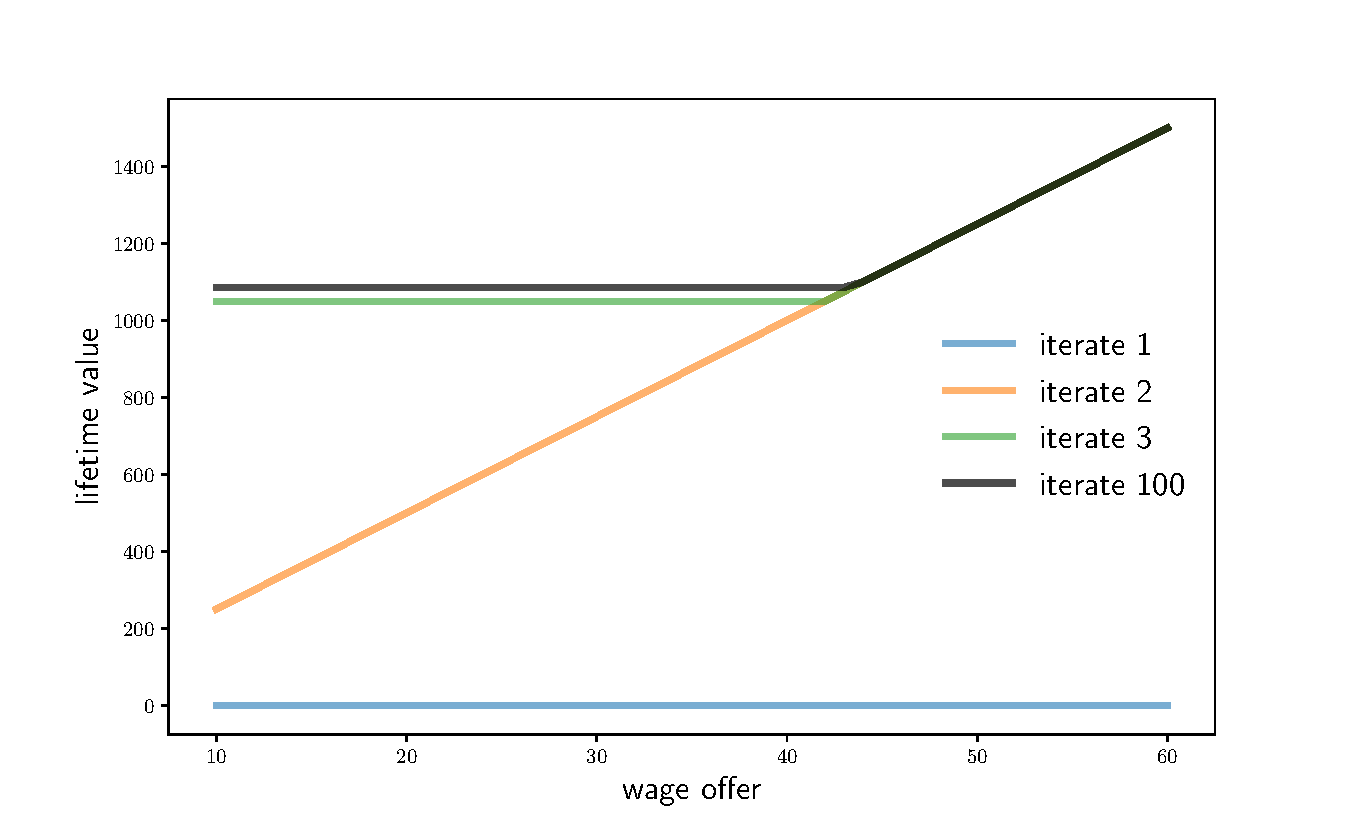
\includegraphics{local_figs/iid_job_search_1.pdf}}
        \caption{\label{f:iid_job_search_1} A sequence of iterates of the Bellman operator}
    \end{figure}
    %


\end{frame}

\begin{frame}

    \begin{figure}
        \centering
        \scalebox{0.42}{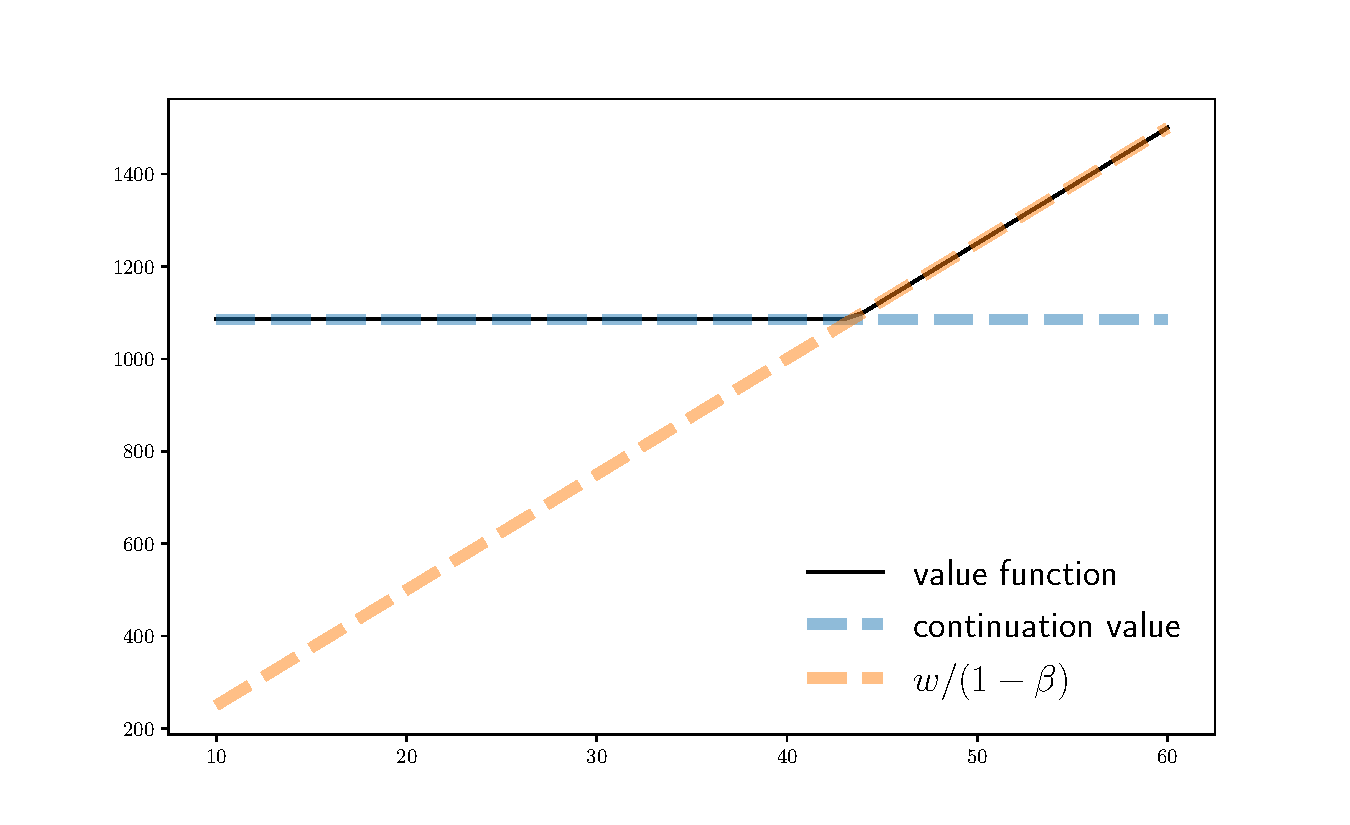
\includegraphics{local_figs/iid_job_search_3.pdf}}
        \caption{\label{f:iid_job_search_3} The approximate value function for job
        search}
    \end{figure}

\end{frame}


\begin{frame}
    \frametitle{Reducing Dimensionality}

    We used VFI because it's standard

            \vspace{0.5em}
            \vspace{0.5em}
    Sometimes we can find more efficient ways to solve particular problems

            \vspace{0.5em}
            \vspace{0.5em}
    In this case we can --- by computing the continuation value directly

            \vspace{0.5em}
            \vspace{0.5em}
    This shifts the problem from $n$-dimensional to one-dimensional

        \vspace{0.5em}
        \vspace{0.5em}
        \emp{Key message:} Look for ways to reduce dimensionality
\end{frame}


\begin{frame}
    
    Method: Recall that 
    %
    \begin{equation*}
        v^*(w) 
        = 
        \max 
        \left\{
            \frac{w}{1-\beta}
            ,\,
            c + \beta \sum_{w'} v^*(w') \phi(w')
        \right\}
        \qquad (w \in \Wsf)
    \end{equation*}
    %

    Using the definition of $h^*$, we can write 
    %
    \begin{equation*}
        v^*(w') = \max \left\{ w'/(1-\beta) ,\, h^* \right\}
        \qquad (w' \in \Wsf)
    \end{equation*}

    Take expectations, multiply by $\beta$ and add $c$ to obtain
    %
    \begin{equation*}
        h^*
        = 
        c + \beta 
        \sum_{w'} \max 
        \left\{
            \frac{w'}{1-\beta}
            ,\,
            h^*
        \right\} \phi(w')
    \end{equation*}

\end{frame}


\begin{frame}

    How to find $h^*$ from the equation
    %
    \begin{equation}\label{eq:cv}
        h^*
        = 
        c + \beta 
        \sum_{w'} \max 
        \left\{
            \frac{w'}{1-\beta}
            ,\,
            h^*
        \right\} \phi(w')
    \end{equation}

    
    We introduce the map $g \colon \RR_+ \to \RR_+$ defined by
    %
    \begin{equation*}
        g(h)
        = 
        c + \beta
        \sum_{w'} \max 
        \left\{
            \frac{w'}{1-\beta}
            ,\,
            h
        \right\} \phi(w')
    \end{equation*}
    %

    By construction, $h^*$ solves \eqref{eq:cv} if and only if $h^*$ is a fixed
    point of $g$  

    \vspace{1em}
    \Ex Show that $g$ is a contraction map on $\RR_+$ 

\end{frame}

\begin{frame}

    \begin{figure}
        \centering
        \scalebox{0.4}{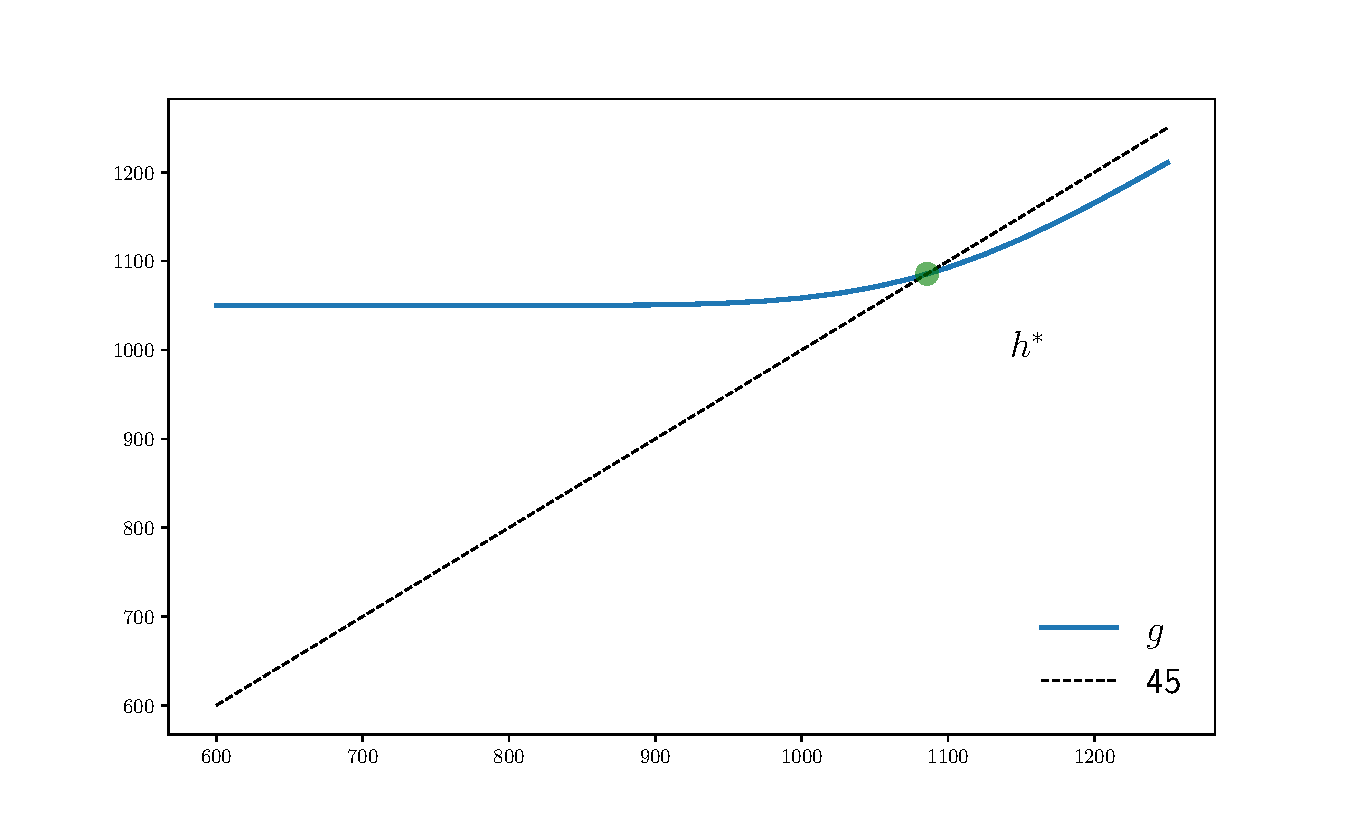
\includegraphics{local_figs/iid_job_search_g.pdf}}
        \caption{\label{f:iid_job_search_4} Computing the continuation value as the fixed point of $g$}
    \end{figure}

\end{frame}


\begin{frame}
    
    New algorithm:

    %
    \begin{enumerate}
        \item Compute $h \approx h^*$ via successive approximation on $g$
            \vspace{1em}
            \begin{itemize}
                \item Iteration in $\RR$, not $\RR^n$
            \end{itemize}
            \vspace{1em}
        \item Optimal policy is 
            %
            \begin{equation*}
                \sigma^*(w)
                = \1
                \left\{
                    \frac{w}{1-\beta}
                    \geq
                    h
                \right\}
            \end{equation*}
    \end{enumerate}


            \vspace{1em}
            \vspace{1em}
    \Ex Implement and compare timing with VFI
            \vspace{1em}


    \begin{itemize}
        \item See the notebook \texttt{job\_search.ipynb}
    \end{itemize}

\end{frame}





\end{document}









